\documentclass[a4paper,11pt,fleqn]{article}%fleqn pour aligner les equations à gauche
\usepackage{../../Styles/Cours}

\newcommand{\chnum}{Chapitre 18}
\newcommand{\chtitle}{Interférences lumineuses}
\newcommand{\dtype}{TP}

  
\begin{document}
\maketitle

\noindent
\fbox{\begin{minipage}[c][5cm][c]{.45\linewidth}
\textbf{Document 1 : Montage}
\begin{center}
    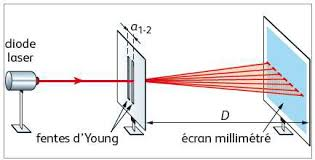
\includegraphics[scale=.7]{Ressources/TSPE_C9_AE3_Fig1.jpeg}
\end{center}
\end{minipage}}
\fbox{\begin{minipage}[c][5cm][t]{.5\linewidth}
\textbf{Document 2 : Interférences}\\
On appelle « fentes de Young » 2 fentes étroites et parallèles de largeur $a$ et distantes l’une de l’autre de $b$.\\
Lorsque la lumière parvient sur ces fentes, celles-ci se comportent alors comme 2 sources en phase et il y a alors interférence entre les 2 sources.
\end{minipage}}

\vspace{.5cm}
\noindent
\fbox{\begin{minipage}{.97\textwidth}
\textbf{Document 3 : Figure d'interférences}\\
On appelle interfrange $i$ la distance en mètre (m) séparant le milieu de 2 franges brillantes ou de 2 franges sombres, consécutives de la figure d’interférence.
\begin{center}
    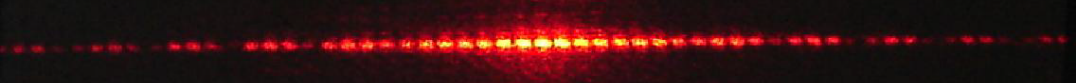
\includegraphics[scale = .45]{Ressources/TSPE_C9_AE3_Fig2.png}
\end{center}
\end{minipage}}

\vspace{.5cm}
\noindent
\fbox{\begin{minipage}{.97\textwidth}
\textbf{Document 4 : Matériel}
\begin{itemize*}
    \item Un Laser produisant une lumière monochromatique de longueur d’onde $\lambda$
    \item Un écran
    \item Un mètre ruban
    \item Une diapositive comportant 3 paires de fentes de Young différentes d’écartement $b$ entre les 2 fentes différent : $b$ = \num{0.20} \unit{\milli\meter}, ou $b$ = \num{0,30}  \unit{\milli\meter} ou $b$ = \num{0,50}  \unit{\milli\meter} (avec $a$ = \num{70}  \unit{\micro\meter})
    \item Une diapositive comportant 4 paires de fentes de Young différentes d’écartement $b$ entre les 2 fentes différent : $b$ = \num{0,25}  \unit{\milli\meter}, ou $b$ =  \num{0,50}  \unit{\milli\meter} ou $b$ = \num{0,75}  \unit{\milli\meter}, ou $b$ = \num{1,00}  \unit{\milli\meter} (avec $a$ = \num{0,15}  \unit{\milli\meter})
    \item Un ordinateur avec le logiciel LatisPro pour traiter et modéliser les mesures.
\end{itemize*}
\end{minipage}}

\vspace{.5cm}
\noindent
\fbox{\begin{minipage}{.97\textwidth}
\textbf{Document 5 : Le CompactDisc}
\begin{multicols}{2}
Le CD permet de stocker des informations numériques, correspondant à \num{650} Mo de données informatiques. Les données sont inscrites sur un seul sillon en spirale, qui fait près de \num{5} \unit{\kilo\meter} de long, du centre vers l’extérieur et 22188 tours. On appelle $e$ le pas du CD qui correspond à l’écartement de la spirale après 1 tour.\\
Le pas du CD (écartement du sillon) est analogue aux fentes de Young ou aux traits d’un réseau. Tout se passe comme s'il s'agissait d'un réseau collé à un miroir. Le phénomène d'interférences sera alors observable par réflexion. On utilise alors le montage suivant >
\columnbreak
\begin{center}
    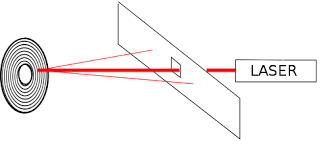
\includegraphics[scale = .7]{Ressources/TSPE_C9_AE3_Fig3.png}
\end{center}
\end{multicols}
\end{minipage}}

\section{Observation du phénomène et mesure de l’interfrange $i$ \emph{(Temps conseillé : 30 min)}}
\begin{enumerate}
    \item Réaliser le montage présenté avec $D$ = \num{1,5} \unit{\meter} et $b$ = \num{0,25} \unit{\milli\meter}. Observer la figure d’interférence obtenue sur l’écran.
    \item Déterminer le plus précisément possible l’interfrange $i$, en explicitant la méthode (un schéma est attendu).
    \item Par analyse dimensionnelle, choisir parmi les formules suivantes, la relation adéquate (homogène) pour l’interfrange $i$ :
    \begin{equationarray}{ccccccc}
        i=D + \dfrac{\lambda}{b} & &i=\dfrac{D\lambda^2}{b} & &i=\dfrac{D\lambda}{b} & & i=\dfrac{D\lambda}{b^2} \nonumber
    \end{equationarray}
    
Avec $b$ la distance séparant les 2 fentes, $D$ la distance fentes–écran et $\lambda$ la longueur d’onde du laser.
\end{enumerate}
\underline{Remarque} : Une relation est homogène (adéquate) lorsque les dimensions des deux membres de l’égalité sont les mêmes.\\

\noindent
\fbox{\begin{minipage}{.95\linewidth}
    \begin{center} 
    Appel professeur n° 1 
    \end{center}
\end{minipage}}

\section{Validation expérimentale du modèle choisi \emph{(Temps conseillé : 60 min)}}

\begin{enumerate}
\setcounter{enumi}{3}
    \item A l’aide du matériel disponible, proposer un protocole permettant de vérifier que l’interfrange $i$ est inversement proportionnelle à l’écartement $b$ des fentes.
\end{enumerate}
\fbox{\begin{minipage}{.95\linewidth}
    \begin{center} 
    Appel professeur n° 2
    \end{center}
\end{minipage}}

\begin{enumerate}
\setcounter{enumi}{4}
    \item Mettre en \oe uvre votre protocole avec $D$ = \num{2,0} \unit{\meter}.
    \item Déterminer la longueur d’onde $\lambda$ de votre Laser.
    \item Valider votre protocole en répondant à la partie 3 de l'activité p. 421 du livre.
\end{enumerate}


\section{Détermination de l’écartement $e$ entre deux branches de la spirale du CD \emph{(Temps conseillé = 20 min)}}
\begin{enumerate}
\setcounter{enumi}{7}
    \item Proposer une méthode et un montage approprié permettant de mesurer l’écartement $e_{TP}$ du sillon.
\end{enumerate}

\noindent
\fbox{\begin{minipage}{.95\linewidth}
    \begin{center} 
    Appel professeur n° 3 
    \end{center}
\end{minipage}}

\begin{enumerate}
\setcounter{enumi}{8}
    \item Mettre en \oe uvre votre protocole.
    \item Donner la valeur de l'écartement $e_{TP}$ (pour les plus rapides : avec son incertitude-type)
\end{enumerate}
\end{document}